\documentclass[a4paper,10pt]{article}
\usepackage[utf8]{inputenc}
\usepackage{fullpage}
\usepackage{mathtools}
\usepackage{graphicx}
\usepackage{insval}
\usepackage{natbib}

\newcommand{\etal}{\textit{et al.}}

\title{Fast inhibitory loop explains functional map development with short-range inhibition.}
\author{J\'an Antol\'ik}

\begin{document}
 \maketitle
\loadkeyvaluestore{/home/jan/Doc/Papers/fast_inh_paper/key_value_store.py}


\section{Introduction}

Competition between populations of neurons has been proposed as one of the canonical computations of cortical 
networks, and has been hypothesized to underly range of brain functions including working memory \cite{Amit1995,Durstewitz2000},
orientation tuning \cite{Somers1995,Ben-Yishai1995}, and functional map development \cite{VonderMalsburg1973,Antolik2011}.
In developmental models of functional cortical organization the competition occurs between populations of neurons spatially offset 
along the cortical surface, and previous studies have shown that a specific arrangement of the effective inhibitory and excitatory 
interactions is required: inhibition has to have longer range than excitation (a so called Mexican-Hat profile) \cite{Muir2014}.
This is, however, in stark contrast to the know anatomical arrangement: the excitatory neurons superficial layers tend to form 
long-range arborizations spanning multiple columns while the axons of majority of inhibitory neurons are confined to area
only several hundreds of micrometers in diameter \cite{Buzas2006,Budd2001}.


As pointed out by Muir et al. in their recent study \cite{Muir2014}, to solve this apparent conflict, previous topologically organized models cortical competition have either relied on the anatomically unsupported Mexican-hat profile of lateral interactions \cite{VonderMalsburg1973,CMVC}, or relied on other biologically unrealistic properties, such as selective targeting of inhibitory neurons by long range excitatory connections \cite{law:phd09,Rutishauser2012} or instantaneous synaptic transmission coupled with omission of recurrent inhibition \cite{Kang2003,Levy2011}. Model analysis by Muir et al. \cite{Muir2014} showed that the presence of competition across the cortical surface is predicted well by the anatomy of direct excitatory and inhibitory coupling and that multi-synaptic network effects are negligible. In conclusion, currently no satisfactory explanation of how topological functional organization dev?lops in cortical networks that is consistent with the present anatomical findings exists. 

All previous topologically organized models of cortical competition have either assumed instantaneous synaptic transmission \cite{VonderMalsburg1973,Kang2003,Levy2011,Grabska-Barwinska2008}} or uniform transmission delays across the different intra-cortical connections \cite{CMVC,Antolik2011}. This is also the case of the analysis performed by Muir et al. \cite{Muir2014} which questions the ability of the accepted cortical architecture to explain cortical competition. However, a recent study by Ohana et al. \cite{Ohana2012} have revealed a specific pattern of transmission delays between different neural type combinations. Specifically they found that the excitatory to excitatory connections are slow while the excitatory to inhibitory connections are fast. In this study we explore the 
possibility that this specific transmission delay pattern is the missing link that can explain how short range inhibition can lead 
to effective cortical competition. We employ computational models to show that the fast excitatory-to-inhibitory-to-excitatory pathway allows for the disynptic inhibition to generate the effective Mexican-hat like lateral interactions, thus for the first time 
explaining competition in topologically organized cortical networks with no biologically implausible assumptions. To demonstrate the
proposed properties, in this study we focus on models of development of orientation maps, because this is the most well explored
example of competition driven functional cortical organization development, but these results generalize to development of other
cortical topological properties, as well as potentially other competition based computations.


\section{Materials and Methods}

Here we describe the two models and their variants used in this study and finish with description of a measure
for assessing the extent to which a model orientation maps resemble their biological counterparts. Since this study heavily leans on methodology 
developed in our previous studies, we offer here only shortened description and refer readers to the original articles for details.


\begin{figure}[htpb!] 
\centering
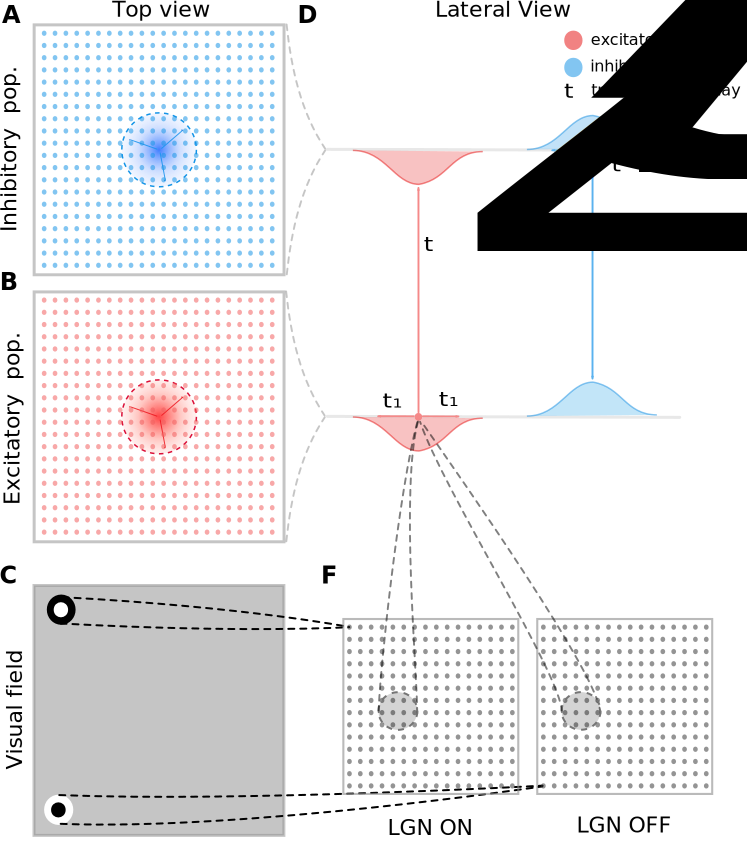
\includegraphics[width=16cm]{./SVG/FigureModelArchitecture/drawing.png}
\caption{General model architecture. (A) Inhibitory cortical population corresponds to a regular lattice of units in cortical space. (B) As in A but 
for excitatory population. (C) Thalamic neurons are modeled as simple difference-of-Gaussian filter followed by a threshold-linear trasfer function. 
(D) The intra-cortical connectivity between the excitatory and inhibitory populations and their transmission delays. The intra-cortical connectivity is the only aspect of the general architecture presented here that changes between the diffrent model variants explored in this study and each variant is detail in figure \ref{fig:model_variants}.
(F) The centers of RFs of the LGN neurons form a regular latice accross the visual space covered by the model. This retinotopic mapping of connection fields between layers of the model is also maintained in the thalamo-cortical projection (lines between D and F)}
\label{fig:model_architecture}
\end{figure} 


\subsection{GCAL model}\label{sec:gcal}

In sections \ref{sec:SM1} through \ref{sec:SM3} we use GCAL model \cite{Stevens2013}  which is the most advanced variant of LISSOM 
(Laterally Interconnected Synergetically Self-Organizing Map) algorithm introduced by Miikkulainen et al. \cite{CMVC}, 
which itself is based on earlier Self-Organizing Map models \cite{Kohonen1982}.

For clarity and consistency the following model description closely follows the methodology sections in our 
previous work \cite{Stevens2013,Antolik2011}. The architecture of the 3 GCAL variants presented in this 
paper is depicted in figure \ref{fig:fig:model_architecture} and figure \ref{model_variants}A-C. The models are implemented in the Topographica simulator, freely available at www.topographica.org. 
Each of the GCAL models consists of set of sheets of model neural units, corresponding to: (1) the photoreceptors, (2) the combined effects of the retinal ganglion cells (RGC) and ON and OFF LGN cells. Furthermore each model has one V1 sheet of units with direct excitatory and inhibitory interactions (section \ref{sec:SM1}), or two 
V1 sheets, one corresponding to excitatory and one to inhibitory neurons (sections \ref{sec:SM2} and \ref{sec:SM3}).
The model sheet is a 2D array of computational elements (called units or, loosely, neurons), with activation and plasticity equations as 
described below and referenced by a coordinate system we will refer to as sheet coordinates, where the center of the sheet is designated (0.0,0.0).  
The number of units simulated in each sheet is determined by the density of units per unit length in both sheet dimensions. 
All cortical sheets have nominal dimensions \insval{cortex_size}$\times$\insval{cortex_size} in sheet coordinates. The sizes of the
RGC/LGN (\insval{lgn_size}$\times$\insval{lgn_size}) and photoreceptor (\insval{visual_field_size}$\times$\insval{visual_field_size}) sheets
were chosen to ensure that each unit in the receiving sheet has a complete set of connections, thus minimizing edge effects in the
RGC/LGN and V1 sheets. The density of units per $1.0\times$1.0 area is \insval{cortex_density}$\times$\insval{cortex_density} 
for the photoreceptor and RGC/LGN ON and OFF sheets, and \insval{cortex_density}$\times$\insval{cortex_density} for both cortical sheets.

\subsubsection{Simulation run-time and stimuly}

As a simplification, GCAL ignores the detailed temporal properties of the sub-cortical neural responses and of signal propagation along the various types of connections. Instead, the model ON/OFF units have a constant, sustained output, and all connections have a constant delay, independent of the physical length of that connection. The simulator operates in discrete time steps. Retinal input changes every \insval{settle_steps} time steps (and during this period is kept constant), and therefore afferent inputs to the V1 sheet(s) are effectively updated every \insval{settle_steps} steps. This process is a discrete simulation of an otherwise continuous series of changes in membrane potential due to incoming spikes and consequent generation of spikes. One such training iteration (\insval{settle_steps} steps) in the model represents one visual fixation i.e., an iteration consists of a constant retinal activation, followed by processing at the ON/OFF and cortical levels.

The activation value $\psi_{i}$ of unit i in the photoreceptor sheet (P) is given by the gray-scale value in the chosen image at that point.
In this study we use two-dimensional elongated Gaussian patterns, who's center coordinates and orientation is sampled from uniform 
distribution that covers the area of photoreceptor sheet and full range of orientations. Each \insval{settle_steps} time steps \insval{num_gaussian_stim} Gaussian patterns are superimposed to form the visual input.

\subsubsection{The LGN/RGC ON and OFF sheets}

The ON/OFF units are called RGC/LGN units because they represent the entire pathway between the retinal photoreceptors
and V1, including the retinal ganglion cells, LGN cells, and the connection pathways. The activation level for a unit at position $j$
in an RGC/LGN sheet at time $t$ is defined as:
%%
\begin{equation}
\eta_{j}(t)=f\left(\frac{A_{j}(t)}{c + \gamma_{L}\sum_{k}A_{k}(t)l_{kj}}\right)
\end{equation}
%%
where
%%
\begin{equation}
A_{j}(t) = \gamma_{F}\sum_{i\in F_j}\Psi_{i}(t)\omega_{ij}
\end{equation}
%%
The activation function $f$ is a half-wave rectifying function that ensures positive activation values, constant $\gamma_{F}=\insval{retina_to_lgn_strength}$ defines the overall strength of the afferent connections from the retina, constant $\gamma_{L}=\insval{lateral_lgn_strength}$ defines the strength of the lateral connections within the RGC/LGN sheet, constant $c=\insval{lateral_lgn_gain}$ defines the slope of the gain, $\Psi_{i}$ is the activation of unit $i$ taken from the set of photoreceptors
from which RGC/LGN unit $j$ receives input (its connection field $F_j$), $\omega_{ij}$ is the connection weight from unit $i$ in the
retina to unit $j$ in the RGC/LGN, and $l_{kj}$ is the lateral connection weight from RGC/LGN unit $k$ to RGC/LGN unit $j$.
Weights from the photoreceptors to units in the ON and OFF channels are set to fixed strengths with a difference-of-Gaussians
kernel ($\sigma_{center}=\insval{lgn_center_sigma}$, $\sigma_{surround}=\insval{lgn_surround_sigma}$, in sheet dimensions), with ON connection fields having a positive center and a negative surround and vice versa for OFF.  The lateral RGC/LGN weights are 2D Gaussians with kernel size $\sigma=\insval{lgn_lateral_sigma}$. The center of the afferent and lateral connection field of each ON/OFF unit is mapped to the location in the photoreceptor and lgn sheet corresponding to the location of that unit in sheet coordinates, making all these projections retinotopic.

\subsubsection{Cortical model}

Units in the cortical sheets each receive three types of projections represented as matrices of weights: afferent excitatory $(p=A)$, 
lateral excitatory $(p=E)$ and lateral inhibitory $(p=I)$.  The contribution $C_{jp}$ to the activation of unit $j$ in a cortical sheet from each projection $p$ at time $t$ is given by: 
\begin{equation} 
C_{jp}(t+\delta t)=\sum_{i\in F_{jp}}\Psi_{i}(t)\omega_{pij} 
\end{equation} 

\noindent where $\Psi_{i}(t)$ is the activation of unit $i$ taken from the set of units in the input
sheet of projection $p$ from which unit $j$ receives input (its connection field $F_{jp}$), and $\omega_{pij}$ is the connection
weight from unit $i$ in the input sheet of projection $p$ to unit $j$ in the in the output sheet of projection $p$. All connection field
weights are initialized with uniform random noise multiplied by a 2D Gaussian profile, cut off at the distance specified below.
Contributions from each projection are weighted and summed and passed via a non-linearity $f$ to calculate the activation of a cortical neuron i at time $t$:
%%
\begin{equation}
\Psi_{i}(t)= f(\sum_{p}\gamma_{p}C_{ip}(t))
\end{equation}
%%
where $\gamma_{p}$ is a constant determining the sign (negative for inhibitory) and strength of projection $p$. 
The transfer function $f$ is a half-wave rectifying function that ensures positive activation values. It has a 
variable threshold point ($\theta$) dependent on the average activity of the unit as described in the next subsection, 
but in all cases the gain is fixed at unity. Table \ref{table:param} shows the strength, initial Gaussian kernel spatial extent, and the cut-off distance values for all projections for the first form of the GCAL model examined in section \ref{sec:SM1}. Any modifications to these base parameters 
in the GCAL model variants examined in sections \ref{sec:SM2} and \ref{sec:SM3} are then reported in the respective sections.

Once all \insval{settle_steps} settling steps are complete, the settled cortical activation pattern is deemed to be the response of cortical sheets to 
the presented pattern. At this point we use the response of cortical neurons to update their threshold point ($\theta$) (using the adaptation process described below) and to update the afferent weights via Hebbian learning. Cortical activity is then reset to zero, and a new pattern is presented. Note that both adaptation and learning could instead be performed at every settling step, but this would greatly decrease computational efficiency.

\subsubsection{Homeostatic adaptation}

The threshold $\theta$ of all cortical excitatory units is updated at the end of each settling phase based on following 
equations:

\begin{equation}
	\theta_{t+1} = \theta_{t} + \xi (\tilde{\Psi}(t) - \mu) 
\end{equation}

where $\xi=\insval{homeostatic_learning_rate}$ is the time constant of the threshold adaptation,
$\mu=\insval{target_activity}$ is a constant defining the target average activity, and $\tilde{\Psi}$ is 
the recent average activity of the unit:

\begin{equation}
  \tilde{\Psi}(t) = (1 - \chi)\Psi(t) + \chi\tilde{\Psi}(t-1)  
\end{equation}

\noindent where $\Psi(t)$ is the output of the unit at time t and $\chi=\insval{activity_average_smoothing}$ is time constant 
controlling the decay of the influence of the past activities. The effect of this scaling mechanism is to bring the average activity of each 
cortical unit closer to the specified target. If the activity in a V1 unit moves away from the target during training, the threshold for activation is thus automatically raised or lowered to bring it closer to the target. Note that an alternative rule with only a single smoothing parameter (rather than
$\xi$ and  $\chi$) could be formulated, but the rule as presented here makes it simple for the modeler to set a desired target activity.

\subsubsection{Hebbian adaptation}

In the model, as images are presented to the photoreceptors, cortical afferent connection weights $\omega_{i,j,A}$ from the ON/OFF sheets are adjusted once per iterations (after cortical settling is completed) using a simple Hebbian learning rule. This rule results in connections that reflect correlations between the presynaptic ON/OFF unit activities and the postsynaptic cortical response. Hebbian connection weight adjustment at each iteration is dependent on the presynaptic activity, the postsynaptic response, and the Hebbian learning rate:

\begin{equation}
\omega_{ijA}(t)=\frac{\omega_{ij}(t-1)+\beta_{p}\Psi_{j}(t)\Psi_{i}(t)}{\sum_{p \in \{ON,OFF\}}\sum_{k}\left(\omega_{kj,p}(t-1)+\beta_{p}\Psi_{j}(t)\Psi_{k}(t)\right)}
\end{equation}

where $\beta_{p}$ is the Hebbian learning rate for the connection fields in the two afferent projections from RGC/LGN $p \in \{\mathrm{ON},\mathrm{OFF}\}$. I.e., the afferent weights from RGC/LGN are normalized jointly.  Learning rate parameters are specified as
a fixed value $\iota_{p}=\insval{learning_rate}$ for each projection, and then the unit-specific values used in the equation above are calculated as
$\beta_{p}=\frac{\iota_{p}}{\upsilon_{p}}$, where $\upsilon_{p}$ is the number of connections per connection field in projection $p$.  


\begin{figure}[htpb!] 
\centering
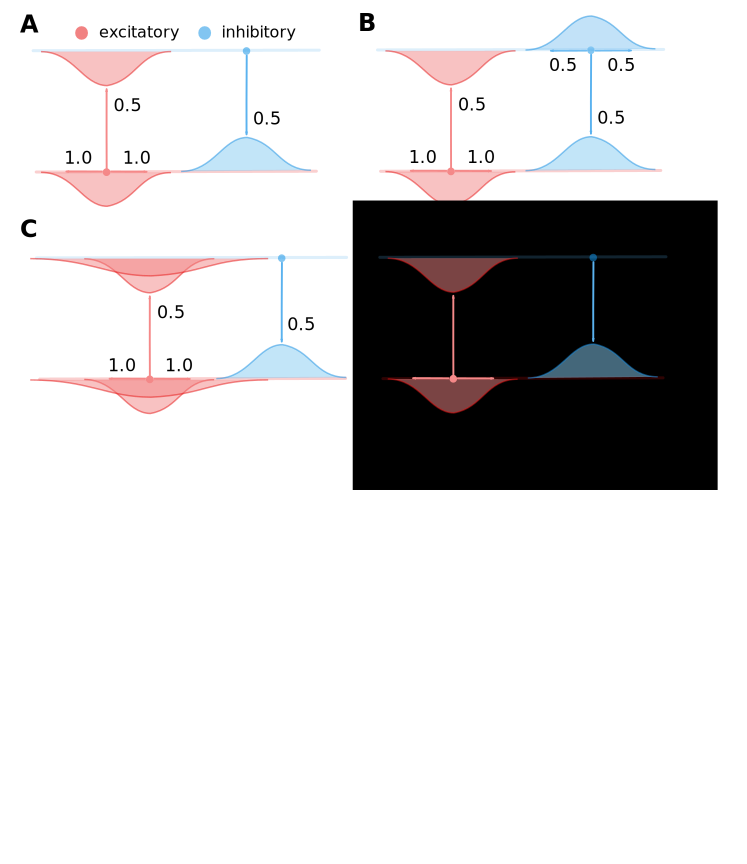
\includegraphics[width=16cm]{./SVG/FigureModelVariants/drawing.png}
\caption{The four considered intra-cortical connectivty variants. (A-C) Are modelled using firing rate models of neural units with instantenous 
translation of inputs into membrane-potential (see section \ref{sec:gcal}). 
(A) Variant 1, assuming only local equaly wide excitatory and inhibitory connectivity, and ignoring direct inhibitory to inhibitory interactions. (B) Variant 2, as in A but with added direct inhibitory to inhibitory connections of equal extent as the other excitatory and inhibitory projections. (C) Variant 3, as in A but with added long-range excitatory connections represented based on Buz\'as \etal\,\cite{Buzas2006} as a second wider gaussian. (D) The same as A but modelled with neural units that take into account membrane time-cosntant (see section \ref{sec:rate}).
The transmission delay of the inhibitory to excitatory projections was varied in the experiments presneted in section \ref{sec:SM4}.}
\label{fig:model_variants}
\end{figure} 


\subsection{Rate model} \label{sec:rate}

The architecture of this model is identical to the GCAL models presented above (see figure \ref{fig:fig:model_architecture}) 
with the exception of the equation ? describing the neural model which is replaced with equation taking into account the 
membrane time constant: 

\begin{equation}
\Psi_{i}(t)= f(\sum_{p}\gamma_{p}C_{ip}(t))
\end{equation}

As a consequence the evolution of the network dynamics have to be simulated at higher resolution. We chose the update step to be ?ms, and we 
let the activity in the model to settle for ?ms, thus resulting in ? settling steps as opposed to the \ref{} of the GCAL model.


figure \ref{fig:fig:model_architecture} and figure \ref{model_variants}A-C

\subsection{Orientation map analysis}

Model orientation maps are calculated based on the vector average method \cite{CMVC}. We first determine the preferred frequency of neurons 
across the map. Due to the simplified stereotypical stimulus used in this study (elongated Gaussian inputs) the spatial frequency 
preference of all neurons lies in a very narrow band, and we thus use the mean preferred spatial frequency across all cortical neurons as the
value for the spatial frequency parameter across all subsequent analysis. Next, sine grating inputs that cover the full range of remaining parameter values (combinations of all orientations and phases) are presented, and for each orientation, the peak response of the neuron is recorded. The orientation preference is calculated by constructing a vector for each orientation $\theta$ (between 0 and 180$\circ$), with the peak response as
the length and $\theta$ as its orientation. These vectors are summed and the preferred orientation is calculated as half of the orientation of the summed vector. The selectivity is given by the magnitude of the summed vector. 

\subsection{Orientation map quality measure}

In order to asses whether the proposed model develops orientation maps that match the structure of those found in real 
animals we need to utilize an automatic metric that tells how close the maps are to animal data. To this end we will 
utilize a map-quality metric that we have recently developed \cite{Stevens2013} based on the empirical observation that pinwheel count 
in biological orientation maps scales linearly with hypercolumn size across many different species \cite{Kaschube2010}.
Specifically the pinwheel density per hypercolumn area ($\Lambda^2$) converges to $\pi$, when averaged across sufficiently 
large cortical surface. For a detailed description of the procedure for calculating this metric we refer reader to 
our previous work \cite{Stevens2013}, but briefly, its calculation involves three steps. First, the locations of the pinwheels
in the orientation map are determined as the intersections of the zero contours of the real and imaginary 
components in the polar representation of the maps, thus yielding the total pinwheel count in the map. Second the 
hypercolumn size is determined as the peak in the isotropic ring-like Fourier transform of the orientation maps.
Third, using these two number we can derive the pinwheel density, but to transform it to a useful metric between 
unity (high-quality map) and zero (low quality map) we pass it through normalized Gama distribution. 
We have shown that this metric reliably distinguishes low and high quality maps \cite{Stevens2013}
and is a valid measure for assessing how well the model orientation maps match animal data.

\section{Results}

In this article we will proceed through multiple gradually more complex models of orientation development, addressing several 
of the major issues with modeling of this phenomena, eventually demonstrating that the experimentally identified fast inhibitory loop is a satisfactory explanation for how short-range inhibition can support development of cortical functional organization. We will use two different computational abstractions to explore the questions at hand. In the fist part of the study we will use computational model that is derived from the LISSOM family of models \cite{CMVC}. This choice has three advantages. It allows for a very straightforward explanation of why 
fast inhibitory loop enables short-range inhibition to induce competition. It makes our explanation directly comparable to the 
extensive set of published LISSOM family models, and thus demonstrates that the solution proposed here generalizes to range of other 
functional properties. And finally the LISSOM abstraction enables very fast simulations, thus allowing us to perform 
parameter search analysis that would be otherwise computationally prohibitive. However, as we will explain further in section \ref{sec:SM4}, some simplifications made by the LISSOM abstraction, specifically the instantaneous translation of the neuronal input into it's activity, will leave 
certain questions unanswered. These will be addressed in section \ref{sec:SM4} using more detailed rate model framework.


\subsection{Fast excitatory to inhibitory to excitatory loop enables competition in networks with short-range inhibitory connections.} \label{sec:SM1}

Ohana et al. \cite{Ohana2012} have shown that transmission delays between different types of cortical neurons are not uniform, specifically they found that on average the transmission delays  between excitatory neurons are $\approx$1.4\,ms, from excitatory to inhibitory neurons are $\approx$0.5\,ms, and from inhibitory to excitatory neurons are $\approx$0.98\,ms. The sample size for connections
between inhibitory cells in the study was not large enough to be quantitatively reliable. The key observation here is that the 
combined di-synaptic delay from excitatory to inhibitory and inhibitory to excitatory cells is approximately as long as the mono-synaptic delay
of the excitatory to excitatory connections. Drawing from this, the core insight of this study is that under such pattern of delays
the effective inhibitory interactions are well approximated by the convolution of the excitatory and inhibitory connection kernels, as we will
show below. This gives the effective inhibition longer range, consequently fulfilling the essential requirement for cortical competition to occur.
For didactic purposes, let us first explore one specific set of conditions under which the above statement holds exactly, we will explore the 
situation when these conditions are relaxed in subsequent sections: 

\begin{enumerate}

\item The sum of the excitatory to inhibitory and inhibitory to excitatory delays is exactly the same as the excitatory to excitatory delay
\item There is no inhibitory to inhibitory interaction
\item The synaptic inputs into the excitatory and inhibitory neurons are instantaneously translated into their rate response via positive rectified transfer function.
\item The connection kernels of all neurons are Gaussian kernels with spatial constant $\sigma_{e}$ for excitatory neurons and $\sigma_{i}$ for inhibitory neurons.
\item We will assume only local connectivity (disregarding long-range excitatory connections), and assume that both excitatory and inhibitory have the same extent, thus $\sigma_{e} = \sigma_{i}$ 
\end{enumerate}

These conditions lead to following set of equations governing the cortico-cortical interaction.
\begin{align}
\label{eqn:first}
\begin{split}
& R_{e}(x,t) = [\sum_{y}N_{\sigma_{e}}(\lVert y-x \rVert)R_{e}(y,t-\theta) - N_{\sigma_{i}}(\lVert y-x \rVert)R_{i}(y,t-\theta) + I_{aff}(x,t)]^+ \\
& R_{i}(x,t) = [\sum_{y}N_{\sigma_{e}}(\lVert y-x \rVert)R_{e}(y,t-\theta)]^+
\end{split}
\end{align}

\noindent where $R_{p}(x,t)$ is the response of neuron of type $p$ located at position $x$ at time $t$, $I_{aff}(x,t)$ is the afferent input to neuron $x$ at time $t$, $N_{\sigma}$
is normal distribution of variance $\sigma$, corresponding to the lateral connection kernel. When we expand for $R_{i}$ we obtain:

\begin{equation}
R_{e}(x,t) = [\sum_{y}N_{\sigma_{e}}(\lVert y-x \rVert)R_{e}(y,t-\alpha) - \sum_{y}N_{\sigma_{i}}(\lVert y-x \rVert)[\sum_{z}N_{\sigma_{e}}(\lVert z-y \rVert)R_{e}(z,t-\theta-\beta)]^+]^+
\end{equation}


\noindent Because $\theta + \beta = \alpha$ (assumption 1) and because the inhibitory neurons receive only excitatory connections (assumption 2) we can further simplify the above as:


\begin{equation}
R_{e}(x,t) = [\sum_{y}N_{\sigma_{e}}(\lVert y-x \rVert)R_{e}(y,t-\alpha) - \sum_{z}\sum_{y}N_{\sigma_{i}}(\lVert y-x \rVert) N_{\sigma_{e}}(\lVert z-y \rVert) R_{e}(z,t-\alpha)]^+
\end{equation}

\noindent and thus due to symmetry of normal distribution:

\begin{equation}
R_{e}(x,t) = [\sum_{y}N_{\sigma_{e}}(\lVert y-x \rVert)R_{e}(y,t-\alpha) - \sum_{z}N_{\sigma_{i}} \ast  N_{\sigma_{e}}(\lVert z-x \rVert) R_{e}(z,t-\alpha)]^+ 
\end{equation}

\noindent Because convolution of two Normal distributions of variance $\sigma_{i}$  and $\sigma_{e}$ is normal distribution with variance $\sqrt{\sigma_{i}^2 + \sigma_{e}^2}$ and 
because $\sigma_{i} = \sigma_{e}$ we can simplify to:

\begin{equation}
\label{eqn:last}
R_{e}(x,t) = [\sum_{y}N_{\sigma_{e}}(\lVert y-x \rVert)R_{e}(y,t-\alpha) - \sum_{z}N_{\sqrt{2}\sigma_{e}}(\lVert z-x \rVert) R_{e}(z,t-\alpha)]^+
\end{equation}

This shows that under these specific assumptions the effective inhibitory interactions between excitatory neurons are $\sqrt{2}$ longer than excitatory and thus follow the Mexican-hat like profile required for for lateral cortical competition underlying functional map development. Even though this essential condition of cortical competition is fulfilled in this model configuration, important constraints on the extent of the effective lateral
interactions (relative to lateral excitation) remain. It is thus still unclear whether development of high-quality orientation maps as observed experimentally is supported under these conditions. Conveniently, the lateral interaction in the LISSOM family of models is governed by the same equations as \ref{eqn:first}. In the following we will use the GCAL model \cite{Stevens2013}, the latest and most robust addition to the LISSOM family of models 
to demonstrate that the above specific configuration of effective lateral excitation and inhibition permits development of high-quality orientation maps. To facilitate comparison we will use exactly the same model configuration 
as in Stevens et al. \cite{Stevens2013} (see Materials and Methods), except to three modifications necessitated by the analysis above:

\begin{enumerate}

\item We will change the spread of lateral inhibition to be $\sqrt{2}$ longer than lateral excitatory spread, such that the resulting lateral
interactions conform with equation \ref{eqn:last}.

\item The change in point 1 will results in change in the balance of overall excitation and inhibition in the model which is critical 
for successful functional development in the model. We will thus modify the strength of the lateral inhibition to compensate for changes due to the modification 1.

\item Analogously to 2, the changes in 1 change the overall balance between feedforward and lateral contributions to model cortical neuron's activity, 
which we will compensate by changing the overall strength of the lateral interactions.

\end{enumerate} 

\begin{figure}[htpb!] 
\centering
\includegraphics[width=16cm]{./SVG/Figure1/figure1.png}
\caption{Orientation map development with short range inhibition and fast excitatory-to-inhibitory-to-excitatory loop. (A) Map quality (see Materials and Methods) at a range of 
lateral excitatory vs inhibitory projection strength ratios and afferent vs lateral projection strength ratios. (B-D) Functional organization in 3 example parameter configurations 
indicated by the red marks. From left to right, the orientation map, fast-Fourier transform of the orientation map and afferent connection fields from the ON LGN model sheet for 25 example model V1 neurons. 
(B-C) Two examples of sub-optimal orientation maps. (D) Model configuration with the highest quality map found in this parameter search. 
(E) The same model configuration but in this case ran with explicit simulation of inhibitory neurons and corresponding connections. E and D are nearly identical confirming correctness of our analysis.
}
\label{fig:figure1}
\end{figure} 


In order to find working combination of parameters in point's 2 and 3, and also to show that the model is robust to certain level of changes
in these two parameters we have performed a parameter search across these two parameters and evaluated the quality of the orientation map (see Materials and Methods) for each 
parameter combination. As figure \ref{fig:figure1} shows, under a range of values of both parameters the model develops high-quality orientation maps indistinguishable
from their experimental counterparts, thus concluding our first step towards showing that fast excitatory-to-inhibitory-to-excitatory loop can explain 
how short-range inhibition can induce cortical competition and consequently development of topological organization of functional properties.

Furthermore, note that the GCAL model used in figure \ref{fig:figure1} only explicitly models excitatory neurons and assumes both direct excitatory and inhibitory
interactions between them, thus corresponding to equation \ref{eqn:last}. Even though above we have shown that equation \ref{eqn:last} is equivalent to equation \ref{eqn:first} to verify 
correctness of our analysis we have ran a single simulation of the GCAL model corresponding to the parameter combination with the highest map 
quality found in figure \ref{fig:figure1}, but with explicitly simulated inhibitory population (figure \ref{fig:figure1}E). In this model we thus do not model direct inhibitory 
interactions between excitatory neurons, but instead add excitatory to inhibitory and inhibitory to excitatory connections of the same extend as those of excitatory to excitatory pathway (see the assumption \#5). 
As we have shown above this model should be mathematically equivalent to the simulations figure \ref{fig:figure1}D. Note, however, that the GCAL simulations represent a discrete approximation 
in both time and space of equations \ref{eqn:first},\ref{eqn:last} and we thus expect small numerical discrepancies. Indeed, orientation maps shown in figure \ref{fig:figure1}E  are nearly identical to those 
in the figure \ref{fig:figure1}D, with only barely perceptible numerical differences, confirming the validity of our approach.


\subsection{Inhibitory to inhibitory connections are consistent with development of functional organization} \label{sec:SM2}

In the previous section we have shown that under a set of specific assumptions short-range inhibition can induce 
effective Mexican-hat like interaction and thus support development of orientation maps. However not all assumptions we 
made were in line with experimental evidence. In this section we will numerically show that one of these assumptions is not necessary, 
specifically that addition of inhibitory connections does not invalidate results of the previous section. 

To this end we will use the exact GCAL model configuration that we have found in previous section to posses the highest
quality orientation map (see figure \ref{fig:figure1}). We will use GCAL configuration in which we will explicitly model the inhibitory neurons
(see figure ?, and equation \ref{eqn:first}) and consequently also explicitly the excitatory to inhibitory and inhibitory to excitatory connections.
Furthermore, we will add inhibitory to inhibitory connections to the model with the same extent as that of inhibitory to excitatory
connections ($\sigma_{i} = \sigma_{e}$ in eq \ref{eqn:first}). 

\begin{figure}[htpb!] 
\centering
\includegraphics[width=16cm]{./SVG/Figure2/figure2.png}
\caption{Orientation map development with short range inhibition, fast excitatory-to-inhibitory-to-excitatory loop and inhibitory to inhibitory connections. (A) Map quality (see Materials and Methods) at a range of 
inhibitory to inhibitory vs inhibitory to excitatory projection strength ratios and excitatory to inhibitory connection strengths. (B-D) Functional organization in 3 example parameter configurations 
indicated by the red marks. From left to right, the orientation map, fast-Fourier transform of the orientation map and afferent connection fields from the ON LGN model sheet for 25 example model V1 neurons. }
\label{fig:figure2}
\end{figure} 

By explicitly modeling the inhibitory neurons in this model we have replaced a single parameter governing the strength of inhibitory
later interactions in the model from previous section with three new parameters that set: (1) strength of excitatory to inhibitory,
(2) inhibitory to excitatory and (3) inhibitory to inhibitory connections (all other parameters remained the same as the 
in the best parametrization found in previous section). Note that in principle there is redundancy in these parameters as
the overall strength of the projections from inhibitory neurons onto both excitatory and inhibitory populations is scaled by the 
excitatory to inhibitory projections strength. Therefore in figure \ref{fig:figure2} we have systematically varied the strength of the added inhibitory to inhibitory
projection expressed relatively to the strength of the inhibitory to inhibitory connections (which was set to 1), while also varying the 
strength of the excitatory to inhibitory projection. We have  investigated the quality of the orientation 
maps that developed under these different levels of inhibitory to inhibitory interactions. As can be seen, high quality maps 
can develop under the full range of the inhibitory to inhibitory interaction strengths, depending on the overall 
excitatory to inhibitory drive. This shows that inclusion of direct inhibitory to inhibitory interactions does not 
invalidate the results of section \ref{sec:SM3}.

\subsection{Long-range excitation} \label{sec:SM3}

In section \ref{sec:SM2} we have only assumed local connectivity by assuming that both excitatory and inhibitory interaction had the same spatial extent. 
However experimental evidence shows that excitatory cells send longer connections compared to inhibitory cells \cite{Buzas2006,Budd2001}. In this section we will
explore what happens if we add long-range excitatory connectivity into the model analyzed in section \ref{sec:SM2}. Buz\'as et al. \cite{Buzas2006} have
shown that the lateral connectivity in layer 2/3 can be best described as superimposition of two gabor connectivity likelyhoods, one short-range not orientation 
specific and one long-range orientation specific. Here we will assume such dual structure, leading us to add second excitatory to excitatory and excitatory to 
inhibitory projection into the model described in section \ref{sec:SM2}, but with 3 times larger space constant (in line with Buz\'as \etal \, \cite{Buzas2006} quantitative findings). 
In figure \ref{fig:figure3} we have  kept the overall strength of excitatory to excitatory and excitatory to inhibitory pathways the same, corresponding to the best 
parametrization found in \ref{sec:SM2}, but varied the relative strength between the short range and long range components (y axis of figure \ref{fig:figure3}). 
Adding the long-range excitation changes the spatial configurations over which excitatory interactions win over inhibitory ones, as well as the 
overall magnitude of the resulting net local excitation. Consequently, the proportion between the magnitude of the net local excitation due to the lateral interactions and the excitation
due to afferent inputs is changed, which is a crucial parameter for map development. To compensate for these changes, we also systematically explore the ratio of the overall magnitudes of the lateral and afferent 
interactions (x axis of figure \ref{fig:figure3}). To make the parameter search computationally feasible, we perform the parameter search only in the region of parameters that allow for sufficiently strong
long-range excitatory projections. As can be seen in figure \ref{fig:figure3}D and E, under appropriately strong lateral interactions, substantial long-range excitatory connection support development of high quality orientation maps, demonstrating that the proposed model is consistent with the experimentally identified long-range excitatory connectivity.

\begin{figure}[htpb!] 
\centering
\includegraphics[width=16cm]{./SVG/Figure3/figure3.png}
\caption{Orientation map development with short range inhibition, fast excitatory-to-inhibitory-to-excitatory loop and long-range excitation. (A) Map quality (see Materials and Methods) at a range of 
short vs. long range excitatory connection strength ratios (y-axis) and range of afferent vs. lateral connection strength ratios (x-axis). (B-E) Functional organization in 4 example parameter configurations 
indicated by the red marks. From left to right, the orientation map, fast-Fourier transform of the orientation map and afferent connection fields from the ON LGN model sheet for 25 example model V1 neurons.}
\label{fig:figure3}
\end{figure} 

\subsection{Non-equal effective excitatory and inhibitory delay} \label{sec:SM4}

In all model variants examined so far we have made the key assumption that the delay on the excitatory to excitatory connections is exactly equal 
to the sum of excitatory to inhibitory and inhibitory to excitatory delays. This assumption is approximately supported by the experimental evidence \cite{Ohana2012}, but we cannot assume it holds exactly in real biological substrate.  However, we hypothesize, that the small discrepancies between the delay of the mono-synaptic excitatory and cumulative delay of the bi-synaptic inhibitory interactions can be absorbed in the membrane time-constant of the neurons. In this section we will verify this hypothesis by extending the modeling framework used thus far with a finite membrane time-constant (see Materials and Methods) and proceed to determine the magnitude of discrepancy in the delays between the excitatory and inhibitory interactions that can be managed by the model without impairing the resulting map orientation map quality. We use model parametrization similar to those determined in previous section \ref{sec:SM1}. For simplicity and computational efficiency we omit the inhibitory to inhibitory and long-range excitatory connections that have already been investigated in sections \ref{sec:SM2} and \ref{sec:SM3}. The membrane time-constant of excitatory neurons was set to \insval{membrane_time_constant_E}ms while those of inhibitory neurons to \insval{membrane_time_constant_I}ms. This faster inhibitory dynamics are necessary to prevent oscillations in the system \cite{Kang2003}. We set the excitatory to excitatory delay to 1.4 ms and excitatory to inhibitory delay to 0.5 ms based on Ohana \etal\,\cite{Ohana2012}. In order to understand how closely does the 
cumulative bi-synaptic inhibition delay has to match that of the direct excitatory to excitatory delay, we will vary the delay on the inhibitory to excitatory projection (note that we could achieve the same by varying excitatory
to inhibitory delay, and this choice was arbitrary). Figure \ref{fig:figure3} shows the resulting orientation maps and associated map quality measures of models with range of differences between the delays of monosynaptic excitatory and bi-synaptic inhibitory interactions, that are in the figure expressed as the sum of the excitatory to inhibitory and inhibitory to excitatory delays. 
 
\begin{figure}[htpb!] 
\centering
\includegraphics[width=16cm]{./SVG/Figure4/figure4.png}
\caption{Orientation map development in a rate model with synaptic time constant. (A) Map quality (see Materials and Methods) at a range of 
cumulative inhibitory delays expressed as the difference from the direct excitatory to excitatory delay. (B-F) Functional organization in 5 parameter configurations 
indicated by the red marks. The orientation map (top), and afferent connection fields from the ON LGN model sheet for 81 example model V1 neurons (bottom). 
(B-D) Three examples of configuration where good quality orientation maps develop. (E) If the cumulative inhibitory delay is longer by more than approximately 0.8ms in comparison
to the direct excitatory delay the map quality starts to drop. (F) In the configuration corresponding to the case where delays on all connections are equal (i.e. the cumulative delay
of the inhibitory interactions is twice as long as on the direct excitatory ones) orientation maps fail to develop.}
\label{fig:figure4}
\end{figure} 

As can be seen when the differences between the excitatory delay (1.4ms) and cumulative inhibitory delay is small (\textless 0.8 ms) high quality orientation maps develop in the model, confirming that sufficiently 
large discrepancy between the direct excitatory and bi-synaptic inhibitory delays can be accommodated in the model. However, as expected, as the difference between the delays increases the ability of the model to learn topological organized representation of orientation preference diminishes. Crucially, if the delays across all the projections would be equal, as is typically assumed, the model fails to develop orientation maps in line with the analysis by Muir \etal \, \cite{Muir2014}, thus confirming that the specific delay pattern between neural types identified by Ohana \etal \, \cite{Ohana2012} is key to achieving competitive dynamics in topologically organized neural models.

\section{Discussion}

In this study we have shown how recent findings on dependence of neural transmission delays on the
type of pre- and post-synaptic neuron \cite{Ohana2012} can resolve long standing question on how short-range inhibition
can support cortical competition and consequently the development cortical functional topological organization.
Under simplifying assumptions, we have analytically shown how dy-synaptic inhibition that is as fast as mono-synaptic 
excitation can extend the effective range of inhibitory interactions, in contrast to the recent analytical 
results showing that in the case of equal synaptic delays on all connections the dy-synaptic inhibition has negligable effects \cite{Muir2014}.\
We have also shown that these findings are applicable to the problem of functional development in primary visual cortex. We have then proceeded 
to show using computational methods that the proposed models are robust to the addition of other well established features of cortical anatomy, commonly 
ignored by similar studies, including the long-range excitatory connections and mutual inhibition among inhibitory neurons. Finally, we have shown 
that the proposed mechanisms are robust to the variations of the exact delay ratio between the mono-synaptic excitation and di-synaptic inhibition. 
Overall, this study represents an important advance in our understanding how orientation map development can be supported by cortical neural substrate. These
results generelize to the development of other functional features in the cortex and other cortical competition based mechanisms in general.

The most related past explanation of how cortical competition can arise under short range inhibition is that of Kang \etal\,\cite{Kang2003}, who have shown 
that under the assumption of faster inibitory time constant (as opposed to excitatory), the effective excitatory and inhibitory interactions will follow the 
Mexican hat profile and thus support competition along the cortical surface. Indeed, in our final model that explicitly considers membrane time-constant presented in section \ref{sec:SM4}, 
we assume that inhibitory neurons have faster membrane time constants than excitatory ones, as otherwise we observe oscilatory behavior in line with the analytical findings of Kang \etal\,\cite{Kang2003}. 
Crucially, Kang \etal\,\cite{Kang2003} however assumed instantenous neural transmission, and when this biologically implausible assumption is rectified by addition of tansmission delays that are uniform 
accross the connections between the different pre- and post-synaptic neural types, we find that the competitive dynamics in the neural model break (section \ref{sec:SM4}E) in line with the analytical and 
computational results of Muir \etal\,\cite{Muir2014}. However, when we replace the tansmission delays with the neural-type specific  pattern uncovered by Ohana \etal\,\cite{Ohana2012} the competitive dymanics 
in the model are rescued and we observe development of high quality orientation maps (section \ref{sec:SM4}AB), in line with the analytical results under simplifieng conditions (section \ref{sec:SM1}).

The analytical results in this study were obtained only under simplifying assumptions, specificaly instantaneous translation of inputs to membrane potential, equal extent of 
excitatory and inhibitory connections and lack of inhibitory-to-inhibitory interactions. Even though we have shown computationally that these assumptions are not neccessary 
for achieving the cortical competition and the consequential orientation map development sought in these study, further analytical work than can circuimvent these simplifications would 
undoubtly provide deeper understanding of the dynamics of the studied neural system and its dependence on the various parameters. This sentiment is underlied by the parameter 
explorations presented here, which show that even though the model is robust to changes of the considered parameters, the existence or not of dynamics supporting development of 
orientation maps forms a complex pattern within the explored parameter spaces. Furthermore, the relative computational complexity of the studied models and the extensive set of parameters
involved preclude systematic search across the full parameter space, and we have only explored parameters that we empirically found to have biggest impact. Finally, one simplifying assumption 
that we have not treated in this study is the lack of direct thalamic input onto inhibitory cells. Since inhibitory cells in cortical layer 4 do receive thalamic input \cite{Binzegger2004} the 
inclusion of external input in the inhibitory population needs to be considered in future.

In this paper we have decided to investigate cortical competitive mechamnisms through the prism of orientation map development. The advantage of this approach is that it allows us not only to show that some form of competition is possible, but also that it is of the form that actually supports implementation of specific cortical computations. 
Given that we show that our model implements effective Mexican hat lateral interactions (section \ref{sec:SM1}) and these have been in the past shown to be sufficient to explain cortical organization of other functional features (i.e. retinotopy, ocular dominance, spatial frequency and color) it is very likely that our results will generalzie to these other dimensions of sensory input as well. Cortical competition of other forms have been proposed to underly broad variety of other cortical operations, including associative memory, noise suppression, decission making, saliency detection and other forms of attentional computations. Even though additional work will be required to determine if the mechanisms proposed here can generelize to these other neural computations, this study offers 
promising framework for anatomically plausible mechinistic explanations of these important aspect of brain function.


\bibliographystyle{abbrv}
\bibliography{./mendeley}

\end{document}



